\section{Structure validation and comparison}
\label{seq:structurevalidation}
 At the end of the refinement process of \ttt{metHgb} $\alpha$ subunit (a similar one would be required for $\beta$ subunit), we need to assess the geometry of our $model$ regarding the starting volume to detect $model$ controversial elements or $model$ parameters that disagree with the map. Although each refinement program has their own tools to assess the progress of refinement (\coot \ttt{Validate} menu; \phenix \ttt{real space refine} real space correlations; \refmac \ttt{R factor} and \ttt{Rms BondLength}), in this tutorial section, three assessment tools will be described to obtain comparative validation values after using any protocol in the workflow:  Protocols \emringer (\scommand{phenix - emringer}, Appendix \ref{app:emRingerProtocol}, \citep{barad2015}), \molprobity (\scommand{phenix - molprobity}, Appendix \ref{app:molprobityProtocol}, \citep{davis2004}), and \validationCryoEM (\scommand{phenix - validation\_cryoem}, Appendix \ref{app:valCryoEMProtocol}, \citep{afonine2018b}). \validationCryoEM protocol will show \molprobity validation values as well as correlation coefficients in real space. Old versions of \phenix (v. 1.13) do not include this tool. Correlation values in real space will thus be computed if a map is provided in \molprobity protocol. Additionally, we are going to introduce the protocol \scommand{phenix - superpose pdbs} (Appendix \ref{app:superposePdbsProtocol}, \citep{zwartUrl}) useful to compare visually the geometry of two atomic structures.\\
 
 Observe some validation steps in the modeling \scipion workflow in \ffigure{fig:scipion_workflow_validation}.

 \begin{figure}[H]
  \centering 
  \captionsetup{width=.9\linewidth} 
  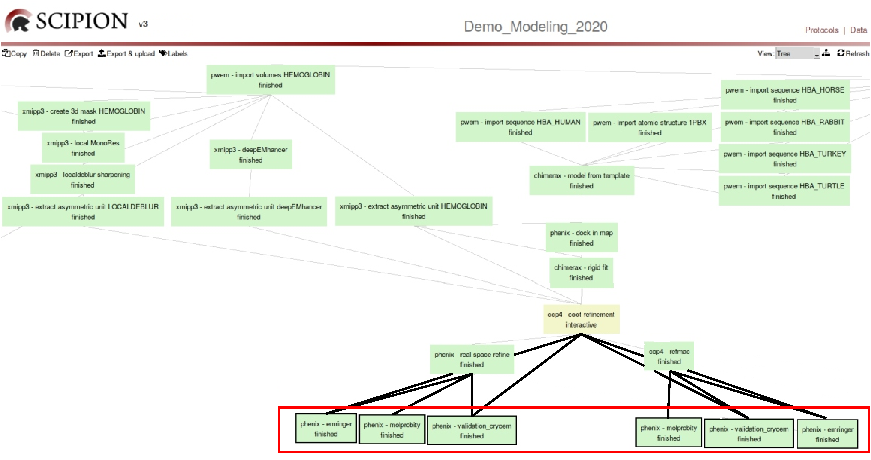
\includegraphics[width=1\textwidth]{Images/Fig69}
  \caption{\scipion framework detailing the workflow to validate the model of the human \ttt{Hgb} $\alpha$ subunit.}
  \label{fig:scipion_workflow_validation}
  \end{figure}
 
 \ttt{Note}: Structure validation is a model building step that you have to perform recursively during the refinement process to assess if you are improving your structure or not. Once you finish the refinement process you'll obtain the final assessment values. These values should be in a certain range if you want to submit the atomic structure to databases. These final validation scores should be computed regarding the density map that you submit as main map, although during the recursive process you might have used the sharpened maps for refinement/validation.


 \subsection*{\emringer}
 
 Specifically designed for cryo-EM data, \emringer tool assesses the appropriate fitting of a model to a map, validating high-resolution features such as side chain arrangements. The placement of side chains regarding the molecule skeleton depends on the $\chi_{1}$ dihedral angle (a dihedral angle is the angle between two intersecting planes), which is determined by atomic positions of (\ttt{N}, \ttt{C$\alpha$}, \ttt{C$\beta$}) and (\ttt{C$\alpha$}, \ttt{C$\beta$}, \ttt{C$\gamma$}) (see \ffigure{fig:emringer_chi1}). The side chain dihedral angles tend to cluster near $180^\circ$ and $\pm60^\circ$. The lower deviations regarding these values, the better $model$, and the higher \emringer value.  

   \begin{figure}[H]
  \centering 
  \captionsetup{width=.9\linewidth} 
  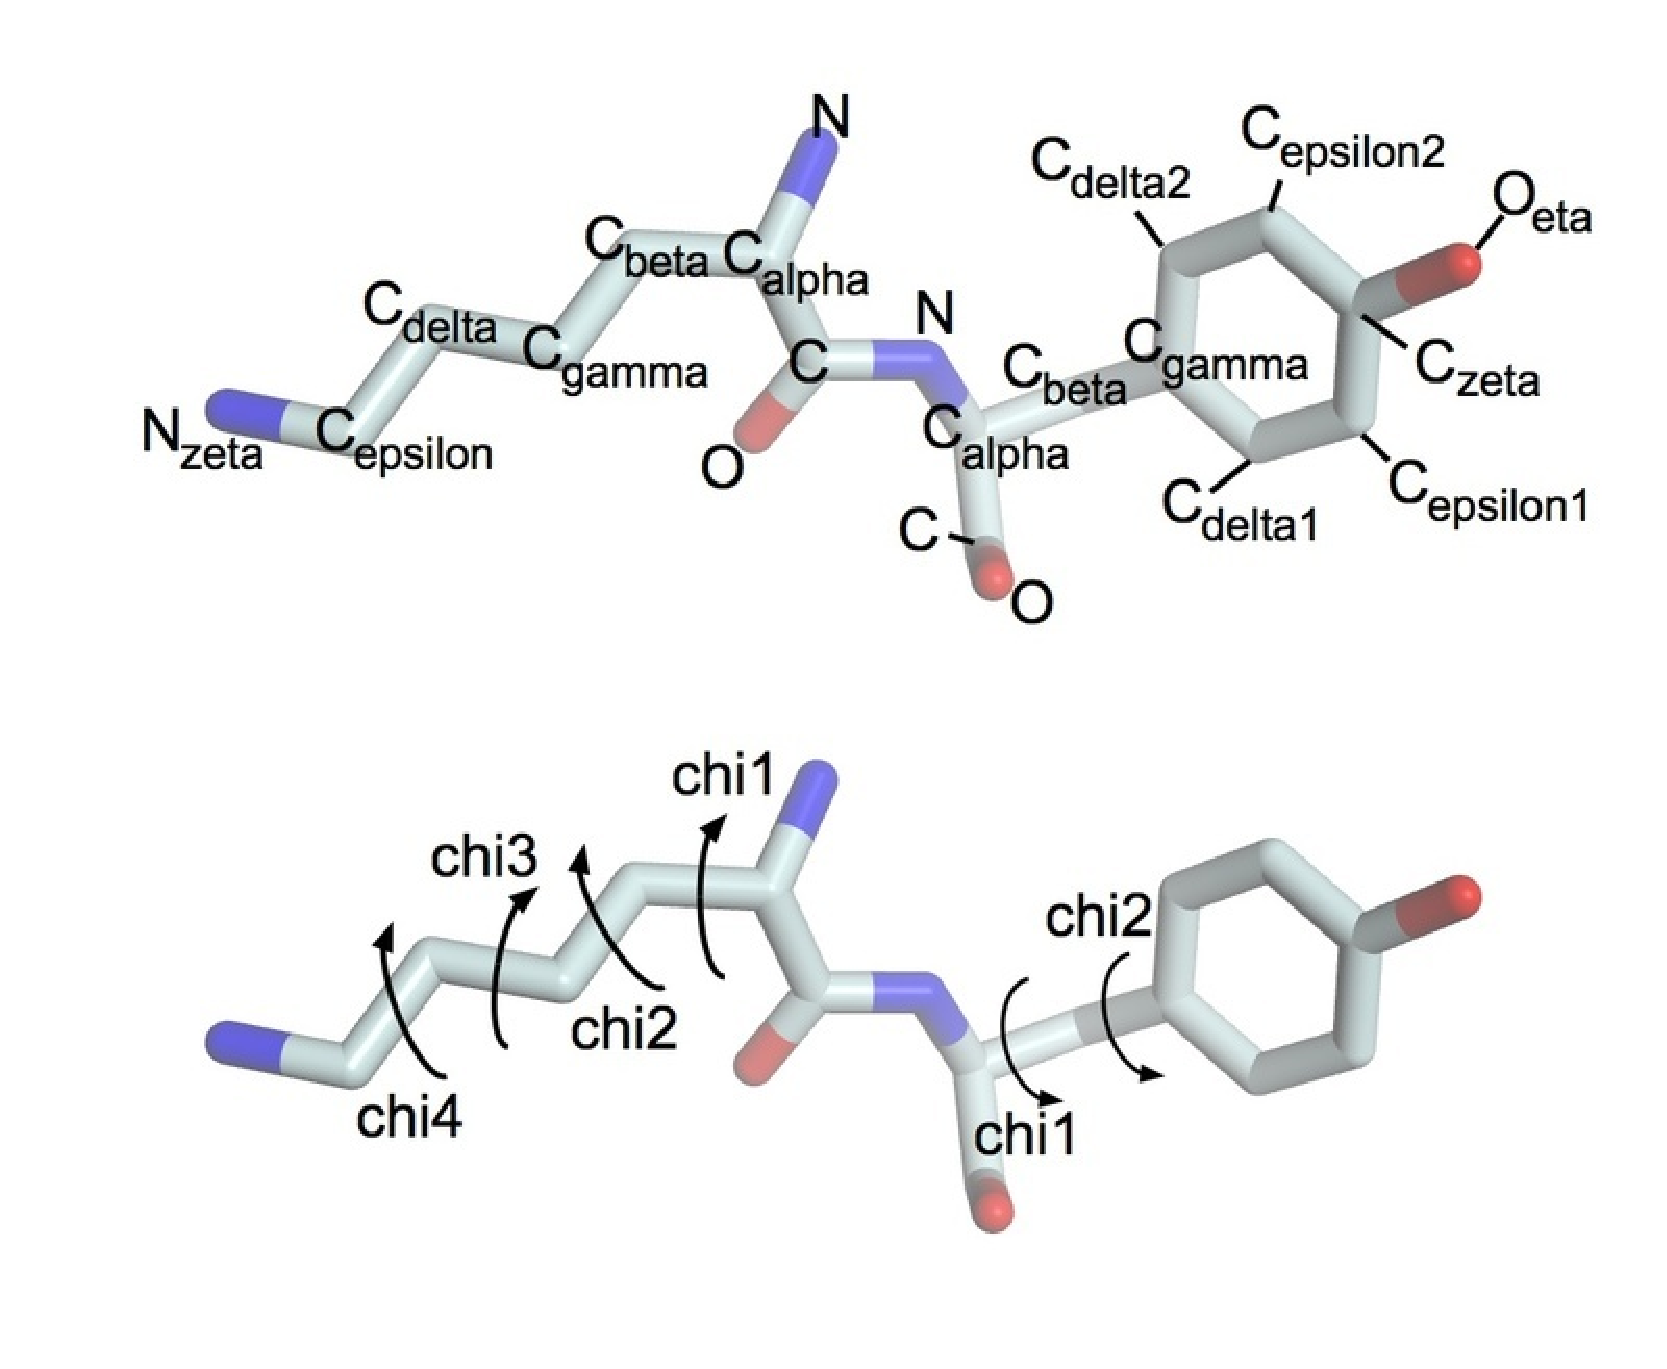
\includegraphics[width=0.65\textwidth]{Images/sidechains}
  \caption{Naming convention in side chains explained in a lysine-tyrosine strand. Note that these two residues are within a protein and thus have no terminal region.}
  \label{fig:emringer_chi1}
  \end{figure}

  
 We can start assessing with \emringer the \ttt{metHgb} $\alpha$ subunit $models$ that we have generated along the modeling workflow. In each case, open the \scommand{phenix - emringer} protocol ((\ffigure{fig:emringer_protocol} (1)), load the extracted map asymmetric unit (initial or saved with \coot) (2) and the atomic structure that you'd like to validate in relation to the map (3), execute the program (4) and analyze results (5). A menu to check results in detail will be opened (bar \ttt{EMRinger results}). \iii{Phenix EMRinger} plots with density thresholds, with rolling window for each chain, as well as dihedral angles for each residue are shown here. The most relevant results, especially the \emringer score, will also be written in the protocol \ttt{SUMMARY} (6). 
 
  \begin{figure}[H]
  \centering 
  \captionsetup{width=.7\linewidth} 
  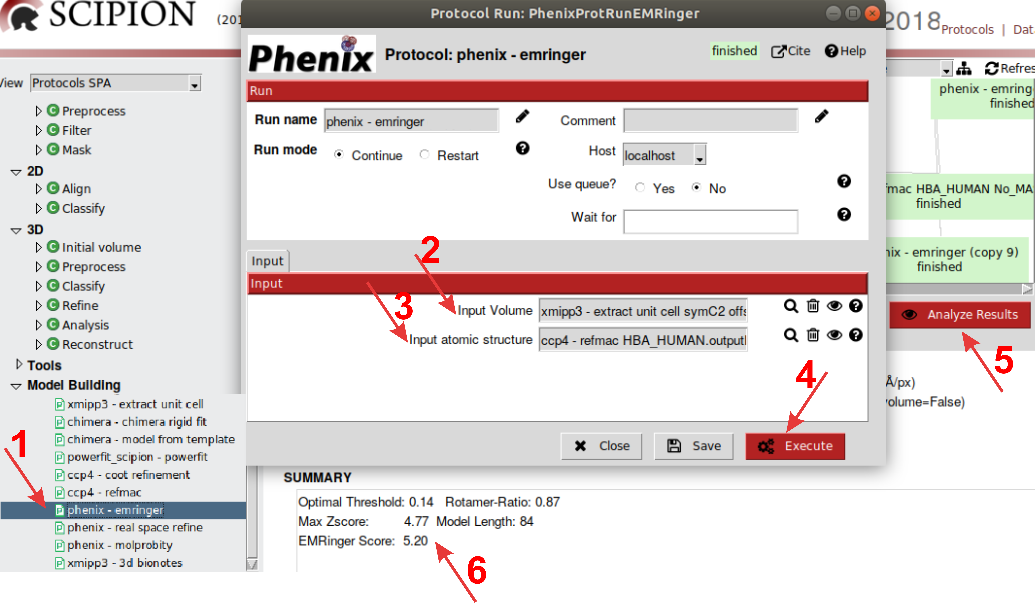
\includegraphics[width=0.85\textwidth]{Images/Fig34}
  \caption{Completing \emringer protocol form.}
  \label{fig:emringer_protocol}
  \end{figure}
 
 Run \emringer protocol and determine the respective score after running \chimera \ttt{rigid fit} , \coot refinement, \phenix \ttt{real space refine} (form parameters indicated in \ffigure{fig:phenix_real_space_refine_protocol}) after \coot, and \refmac refinement with MASK before and after \phenix \ttt{real space refine}. Considering \emringer \ttt{score}, does our \ttt{metHgb} $\alpha$ subunit $models$ seem to be OK or, at least, have they been improved? (Answers in appendix \ref{app:solutions}; \textbf{Question \ref{seq:structurevalidation}\_1}). Try the same validation with $\beta$ subunit $models$. \\
 %[** EMringer results Roling windows does not work]
 
 \subsection*{\molprobity}
 
 The atomic structure validation web service \molprobity, with better reference data has been implemented in the open-source CCTBX portion of \phenix \citep{williams2018}. This widely used tool assesses $model$ geometry and quality at both global and local levels. Originally designed to evaluate structures coming from X-Ray diffraction and NMR, it does not take into account the quality of the fitting with a 3D density map.  The implementation of \molprobity in \phenix v. 1.13, nevertheless, includes the possibility of adding a volume and assessing the correlation in the real space.\\
 
 The assessment process that we have carried out with \emringer can also be done with \molprobity in \scipion. We are going to validate the geometry of \ttt{metHgb} $\alpha$ subunit $models$ that we have generated along the modeling workflow. In each case, open the \scommand{phenix - molprobity} protocol (\ffigure{fig:molprobity_protocol} (1)), load the extracted unit cell volume (initial or generated by \coot) (2) with its resolution (3) only if your \phenix version is 1.13 and you want to have real space correlation between map and $model$. For \phenix versions higher than 1.13 simply load the $model$ atomic structure (4) and execute the protocol (5). With \ttt{Analyze results} (6) menu bars are shown. \molprobity results bar include validation statistics. Protocol \ttt{SUMMARY} emphasizes the most relevant ones (7).\\
 
 \begin{figure}[H]
  \centering 
  \captionsetup{width=.7\linewidth} 
  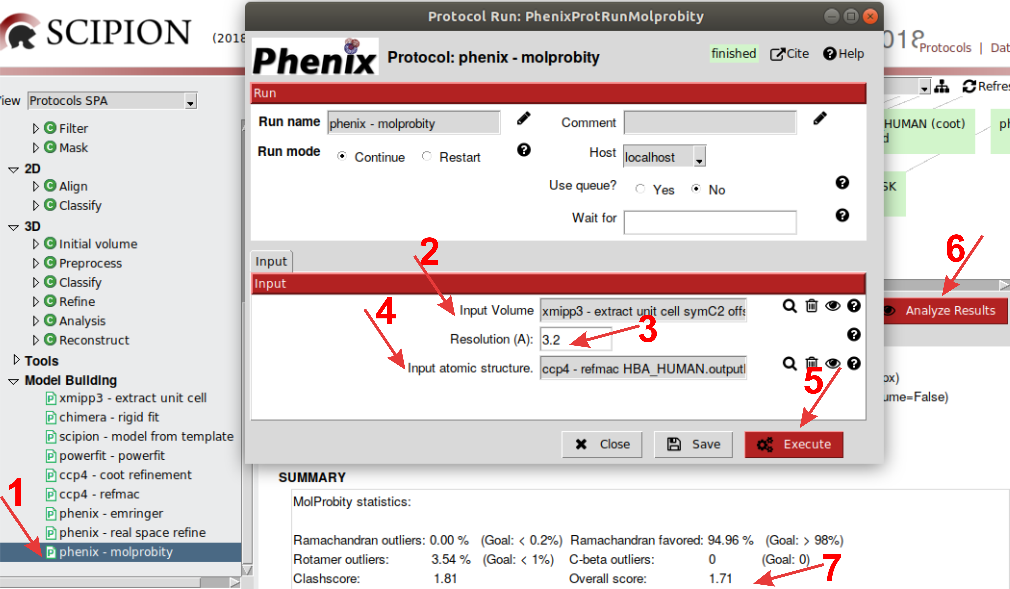
\includegraphics[width=0.85\textwidth]{Images/Fig35}
  \caption{Completing \molprobity protocol form.}
  \label{fig:molprobity_protocol}
  \end{figure}
  
  Run \molprobity protocol to obtain its statistics after running \chimera \ttt{rigid fit}, \coot refinement, \phenix \ttt{real space refine} (form parameters indicated in \ffigure{fig:phenix_real_space_refine_protocol}) after \coot, and \refmac refinement with MASK before and after \phenix \ttt{real space refine}. 
  
  \subsection*{\validationCryoEM}
  
  \phenix versions higher than 1.13 combine multiple tools for validating cryo-EM maps and models into the single tool called \validationCryoEM (\citep{afonine2018b}). This tool has been implemented in \phenix versions higher than 1.13.\\
  
  To carry out the global validation of maps and models obtained from cryo-EM data, open the protocol \scommand{phenix - validation\_cryoem} in \scipion (\ffigure{fig:validationCryoEM_protocol} (1)), load the map (initial or generated by \coot) (2) with its resolution (3), load the $model$ atomic structure (4) and execute the protocol (5). \ttt{Analyze results} (6) shows the same menu bars available in results section of \phenix \ttt{real space refine} protocol. \molprobity results bar include validation statistics. Protocol \ttt{SUMMARY} (7) emphasizes the most relevant ones.\\
  
  \begin{figure}[H]
    \centering 
    \captionsetup{width=.7\linewidth} 
    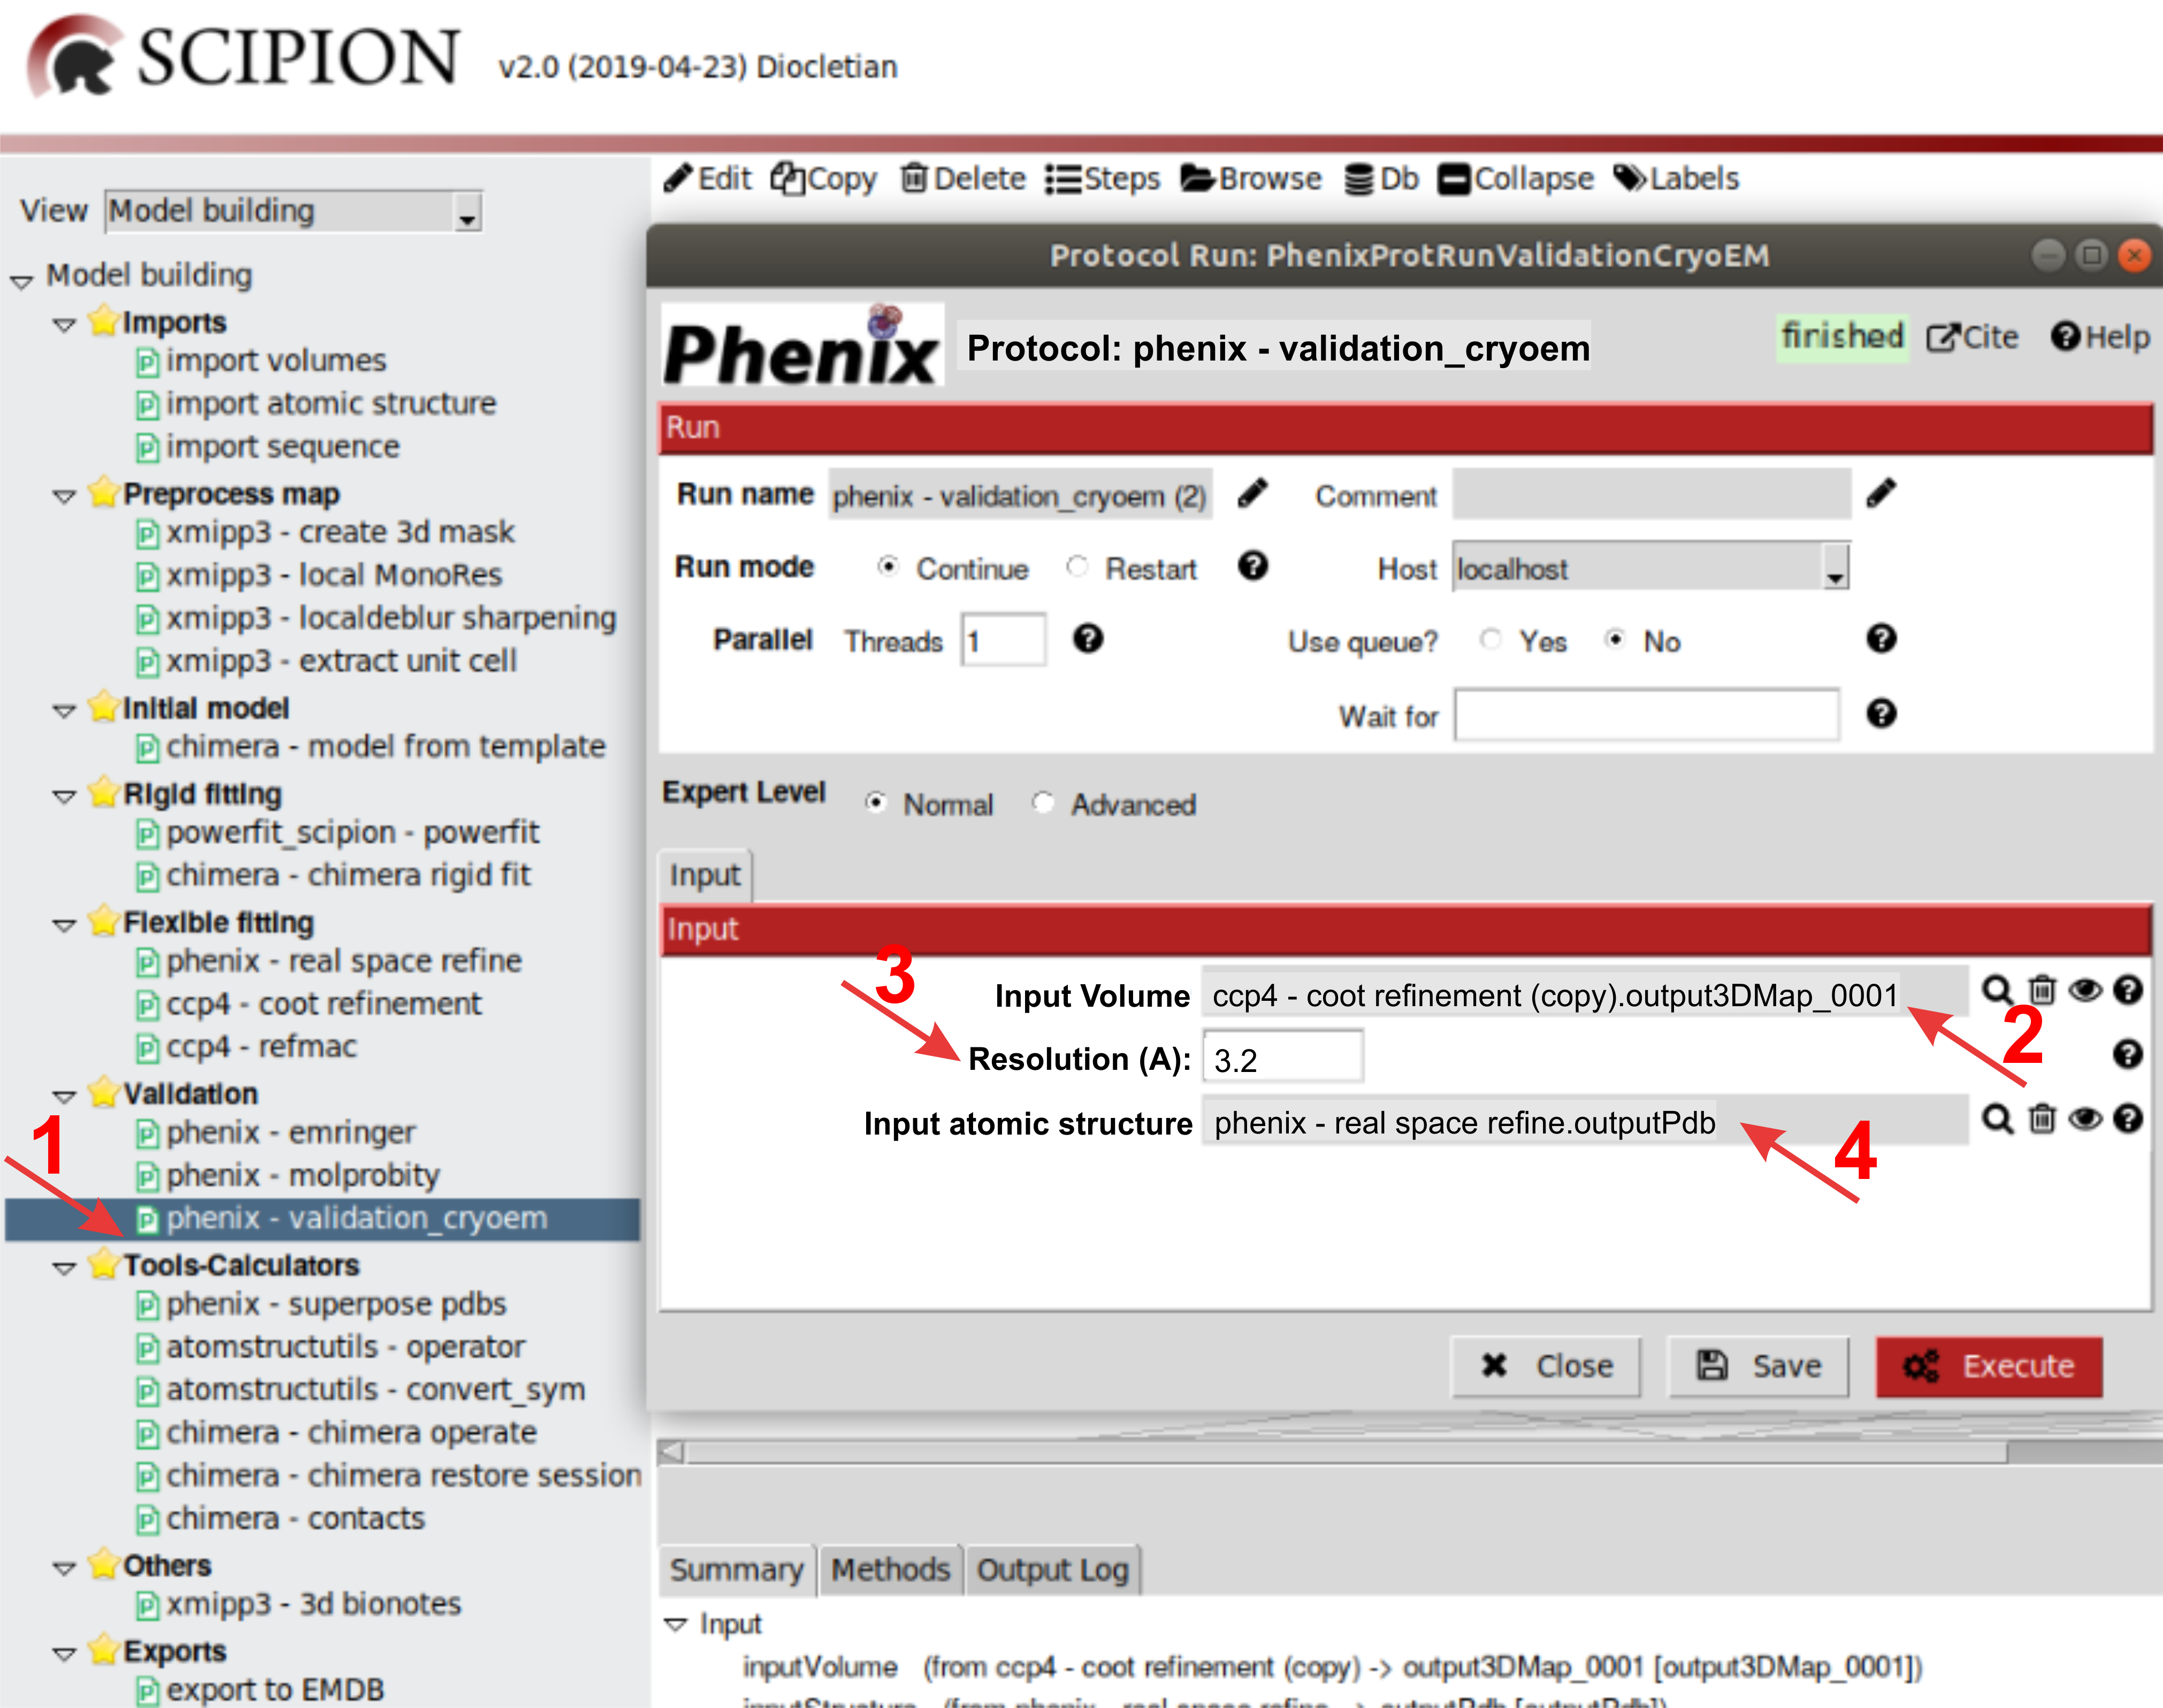
\includegraphics[width=0.90\textwidth]{Images/Fig60}
    \caption{Filling in \phenix \validationCryoEM protocol form.}
    \label{fig:validationCryoEM_protocol}
    \end{figure}
  
  In order to compare validation results of $models$ obtained along the modeling workflow, fill in the next table (\ttable{table:empty}) including, in addition to \molprobity statistics, \emringer scores and \ccmask values obtained before. (Answers in appendix \ref{app:solutions}; \textbf{Question \ref{seq:structurevalidation}\_2}). The same table (\ttable{table:empty}) can be completed for \ttt{metHgb} $\beta$ subunit (Appendix \ref{app:solutions}; \textbf{Question \ref{seq:structurevalidation}\_3})\\
  
 \begin{table}[H]
   \caption{Validation statistics of human \ttt{metHgb} $\alpha$ subunit $model$. \ttt{RSRAC} stands for \ttt{Real Space Refine} after \coot. \ttt{Rama} stands for \ttt{Ramachandran}.}
   \centering\footnotesize
   \begin{tabular}{l c c c c c c }
   \hline\hline
   Statistic &  \chimera & \coot & \thead{\phenix\\ \ttt{RSRAC}} & \thead{\refmac\\ after \coot} & \thead{\refmac\\ after \ttt{RSRAC}} & \ttt{5NI1}\\ [0.5ex]
   \hline
   \ccmask \\
   \emringer \ttt{score} \\
   \ttt{RMS} (Bonds) \\
   \ttt{RMS} (Angles) \\
   \ttt{Rama favored} (\%) \\
   \ttt{Rama allowed} (\%) \\
   \ttt{Rama outliers} (\%) \\
   \ttt{Rotamer outliers} (\%) \\
   \ttt{Clashscore} \\
   \ttt{Overall score} \\
   \ttt{C$\beta$ deviations} \\
   \ttt{RMSD} \\[1ex] 
   \hline
   \end{tabular}
   \label{table:empty}
   \end{table}
 
 
 Results compiled in this table indicate that statistics are uncorrelated. From the point of view of correlation in real space, the best $model$ was obtained from \phenix \ttt{real space refine} after \coot. Considering \emringer \ttt{score}, the best $model$ derives from the whole workflow \coot \ttt{->} \phenix \ttt{real space refine}. With \molprobity \ttt{Overall score} as validation rule, the last step in the workflow could be suppressed because the best value was obtained after \coot \ttt{->} \phenix \ttt{real space refine} (last modification of parameters). We'd like to select the best $model$ and continue refining it in order to improve it as much as possible. Assuming that no one $model$ is perfect, how can we select the best one?\\ 


 \subsection*{$Model$ Comparison}
 
 The question posed in the previous item does not have an easy answer in the real world, in which we do not know the final atomic structure. In this tutorial, nevertheless, we know the atomic structure already published for this cryo-EM map and we may wonder how far we are from it. The question can be answered by comparing a) validation statistics that we have obtained for our $models$ with the statistics computed for the available $\alpha$ subunit in \ttt{PDB} structure \ttt{5NI1}, and b) the atomic structures themselves by overlapping.
    
  \subsubsection*{Comparison of validation statistics}
  
  Validation statistics of \ttt{metHgb} $\alpha$ subunit of \ttt{PDB} structure \ttt{5NI1} should be obtained as first step to compare them with validation statistics of our $models$. With this aim we are going to follow the next workflow:
  
  \begin{itemize}
    \item Protocol \scommand{import atomic structure}:\\
    Download from \ttt{PDB} structure \ttt{5NI1}\\
    
    \item Protocol \scommand{chimera operate} (Appendix \ref{app:chimeraOperate}):\\
    Similar to \chimera \ttt{rigid fit}, \chimera \ttt{operate} protocol allows to perform operations with atomic structures. We are going to use this protocol to save independently in \scipion the \ttt{metHgb} $\alpha$ subunit. Open the protocol  (\ffigure{fig:chimera_operate_protocol} (1)), complete the parameter \ttt{PDBx/mmCIF} including the atomic structure \ttt{5NI1} previously imported (2), and execute the protocol (3).      
    
    \begin{figure}[H]
    \centering 
    \captionsetup{width=.7\linewidth} 
    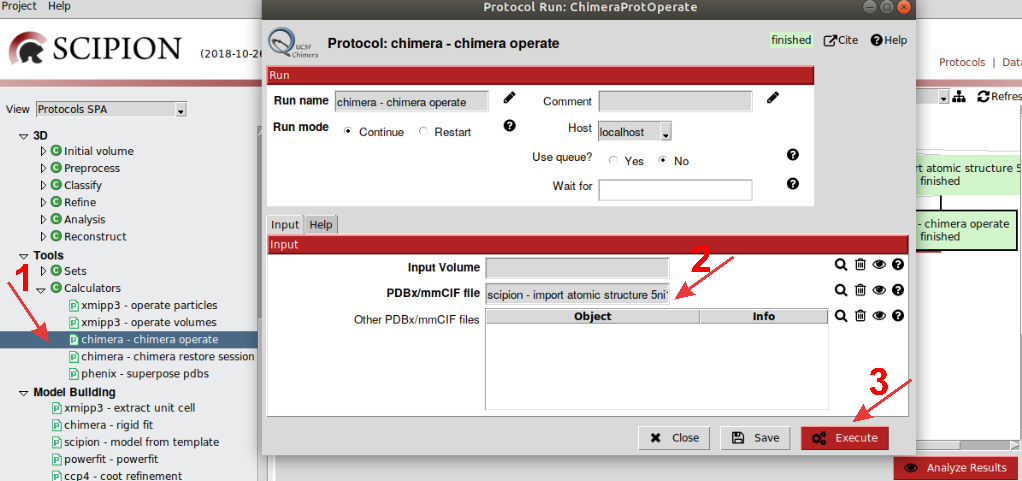
\includegraphics[width=0.90\textwidth]{Images/Fig36}
    \caption{Filling in \chimera \ttt{operate} protocol form.}
    \label{fig:chimera_operate_protocol}
    \end{figure}
    
    The \chimera graphics window will be opened with the structure \ttt{5NI1} as model number \#1. To save independently the structure of human \ttt{metHgb} $\alpha$ subunit (chain A), write in \chimera command line:\\
    \ttt{split \#2}\\
    \ttt{rename \#2.1 id \#3}\\
    \ttt{scipionwrite \#3 prefix 5ni1\_chainA\_}\\
    
    Remark that the model saved in \chimera command line includes both the aminoacid chain and the \ttt{HEME} group. In case you are interested in extracting only the aminoacid chain, you can use the protocol \scommand{atomstructutils - operator}, specifically designed to extract/add individual chains from/to an atomic structure (Atomic Structure Chain Operator; Appendix \ref{app:atomStructUtilsOperatorProtocol}). Compare the results of protocols \chimera \ttt{operate} and Atomic Structure Chain Operator in \ffigure{fig:chimera_operate_protocol_2}. The red arrow points at \ttt{HEME} group.
    
    \begin{figure}[H]
    \centering 
    \captionsetup{width=.9\linewidth} 
    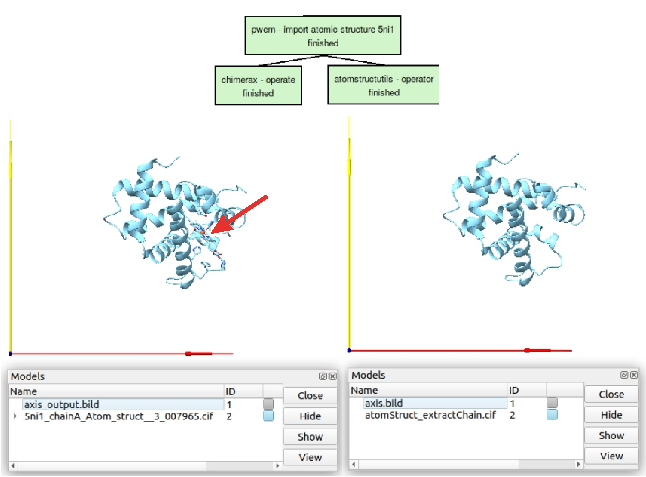
\includegraphics[width=0.75\textwidth]{Images/Fig70}
    \caption{Comparison of results obtained with the protocols \chimera \ttt{operate} (left) and Atomic Structure Chain Operator (right).}
    \label{fig:chimera_operate_protocol_2}
    \end{figure}
    
    \item Protocol \scommand{powerfit}:
    
    Open \powerfit protocol and follow the instructions above indicated. The structure saved in \chimera operate will replace this time our previous $model$ (). Select \ttt{item 2} as best fit.\\
    
    \item Protocol \scommand{chimera rigid fit}:
    Open again \chimera \ttt{rigid fit} protocol and, following already indicated instructions, include this time \ttt{item 2}, the last fitted structure obtained with \powerfit (\ffigure{fig:chimera_rigid_fit} (3)). After finishing the rigid fit of the extracted unit cell and \ttt{metHgb} $\alpha$ subunit from 5NI1 structure, you can save this fitted structure writing in \chimera command line:\\
    \ttt{scipionwrite model \#2 refmodel \#1 saverefmodel 0}\\
    
    \item{Validation protocols \scommand{phenix - emringer} and \scommand{phenix - validation\_cryoem} (\scommand{phenix - molprobity} for \phenix version 1.13)}:
    
    Compute validation statistics with these two protocols for \ttt{metHgb} $\alpha$ subunit from \ttt{PDB} structure \ttt{5NI1}, write respective values in the previous table (\ttable{table:empty}), and compare them with the statistics of our $models$.
    
    Considering results shown in appendix \ref{app:solutions} (\textbf{Question \ref{seq:structurevalidation}\_2}) for \ttt{metHgb} $\alpha$ subunit, we can conclude that published structures are not perfect and we are not very far from this published one. In fact, we have overcome every statistic except \ccmask. Nevertheless, the different $models$ generated after \coot refinement can still be improved by iterative refinement processes. Validation statistics thus allow to follow the quality improvement of atomic models.\\

 
  \subsection*{Comparison of atomic structures}
  
  \phenix protocol \scommand{phenix - superpose pdbs} allows to compare two atomic structures by overlapping them. Root mean square deviation (RMSD) between the fixed structure (the published one) and one of our $models$ supports the classification of $models$ according to its proximity to the published model. Open \phenix \ttt{superpose pdbs} protocol form (\ffigure{fig:superpose_pdbs_protocol} (1)), include the published structure of the \ttt{metHgb} $\alpha$ subunit as fixed structure (2), each one of the $models$ generated along the worflow (3) and execute the protocol (4). Finally, complete the \ttable{table:empty} with the value of RMSD obtained for each $model$. (Answers in appendix \ref{app:solutions}; \textbf{Question \ref{seq:structurevalidation}\_2}).
  
  \begin{figure}[H]
    \centering 
    \captionsetup{width=.7\linewidth} 
    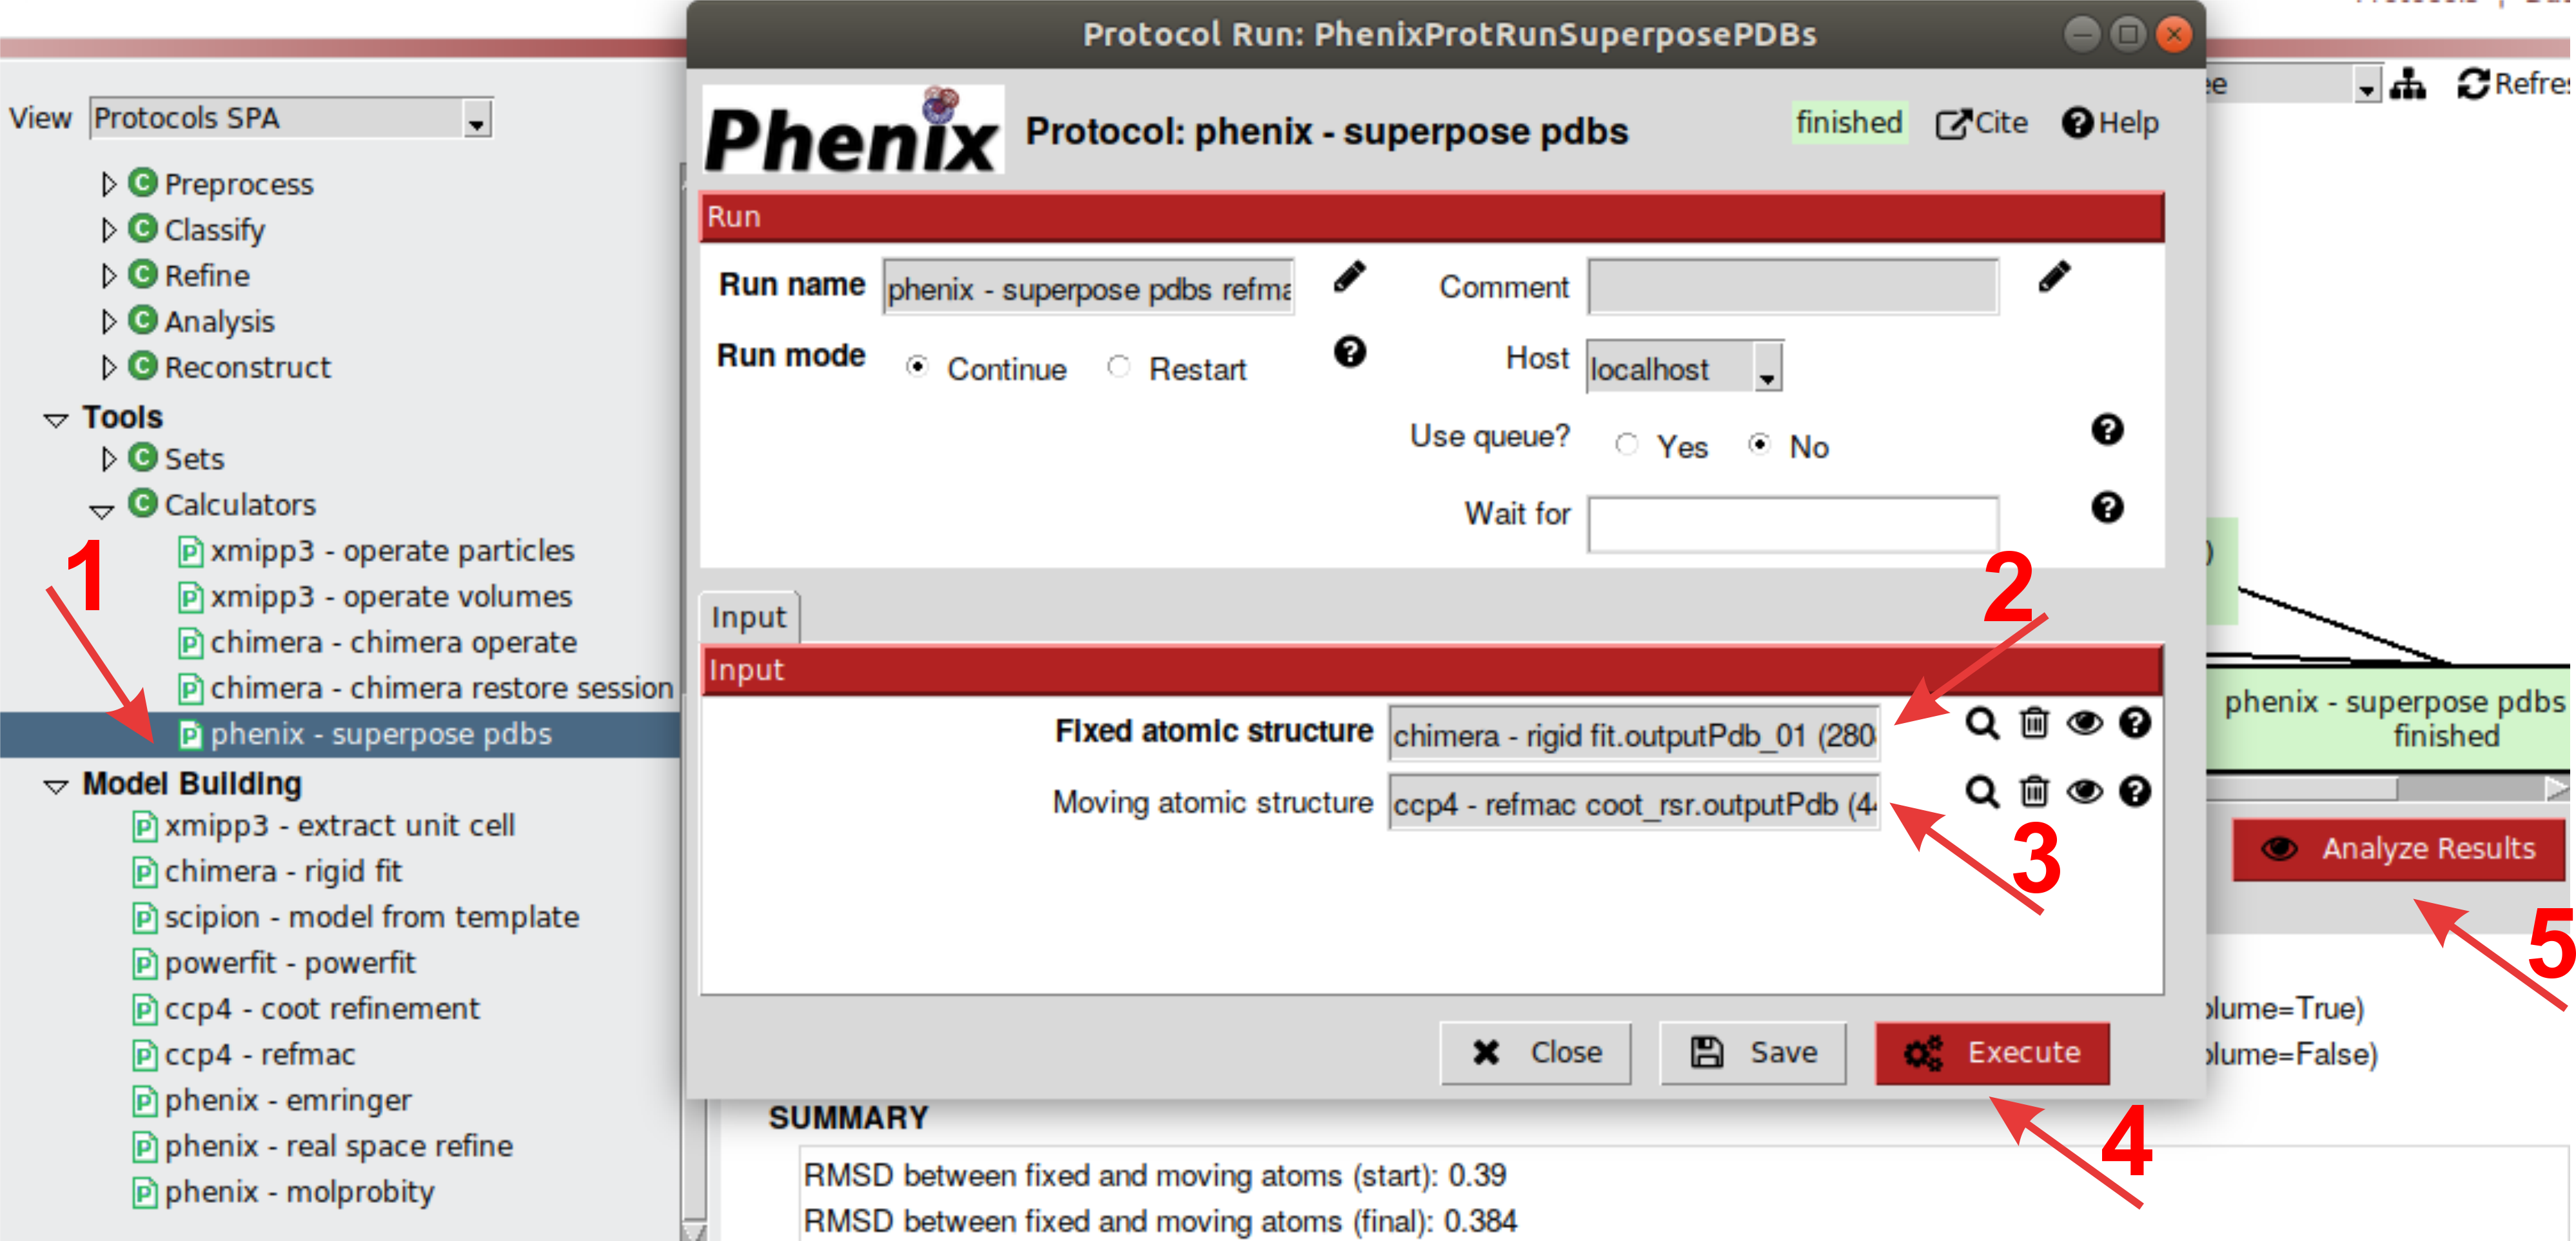
\includegraphics[width=0.90\textwidth]{Images/Fig37}
    \caption{Completing \phenix \ttt{superpose pdbs} protocol form.}
    \label{fig:superpose_pdbs_protocol}
    \end{figure}
    
  You can check in \chimera the fitted $model$ to the published structure by pressing \ttt{Analyze results} (\ffigure{fig:superpose_pdbs_protocol} (5)). Arrows of \ffigure{fig:superpose_pdbs_chimera} remark differing parts between both atomic structures. By opening these structures in \coot you can see the difference between them.
 
   \begin{figure}[H]
    \centering 
    \captionsetup{width=.7\linewidth} 
    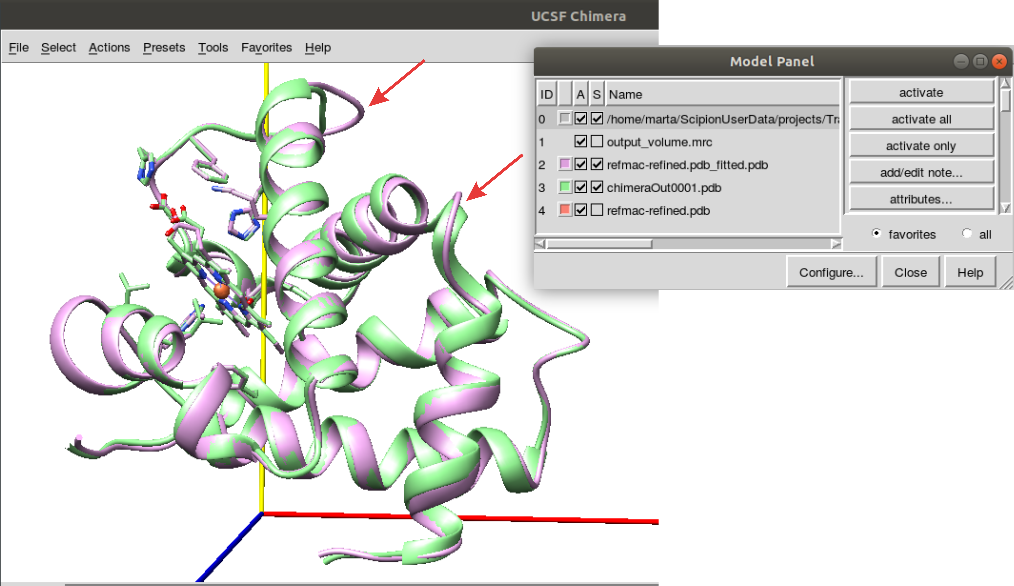
\includegraphics[width=0.70\textwidth]{Images/Fig38}
    \caption{$Model$ generated for \ttt{metHgb} $\alpha$ subunit superposed to published $\alpha$ chain of \ttt{5NI1} structure.}
    \label{fig:superpose_pdbs_chimera}
   \end{figure}
  
  
  \end{itemize}
 
 A $model$ for \ttt{metHgb} $\alpha$ subunit has to be selected at the end of validation process. According to the statistics of \ttable{table:refmac_question_9} (Appendix \ref{app:solutions}; \textbf{Question \ref{seq:structurevalidation}\_2}), $model$ obtained in the last step of modeling workflow (\refmac after RSRAC (modified)) has been selected due to the smallest RMSD value, high value of \emringer \ttt{score}, quite high value of \ccmask and acceptable \molprobity statistics. Follow a similar process to validate and select the $model$ generated for \ttt{metHgb} $\beta$ subunit. Appendix \ref{app:solutions} \textbf{Question \ref{seq:structurevalidation}\_3} contains a statistics table for \ttt{metHgb} $\beta$ subunit, similar to that obtained for \ttt{metHgb} $\alpha$ subunit.\\
 
 In the real world selected $models$ usually are the starting point to improve specific validation parameters by additional refinement. Since the improvement of certain parameters normally implies worsening of other parameters, a final compromise solution has to be taken.\\

